\documentclass[aps,prl,twocolumn,groupedaddress]{revtex4-1}
% \documentclass[aps,twocolumn,secnumarabic,balancelastpage,amsmath,amssymb,nofootinbib]{revtex4-1}
\usepackage{amsmath}
\usepackage{amssymb}
\usepackage{amsfonts}
\usepackage{chapterbib}
\usepackage{color}
\usepackage{graphics}
\usepackage[pdftex]{graphicx}
\usepackage[utf8x]{inputenc}
\usepackage[colorlinks=true]{hyperref}

\newcommand{\ud}{\mathrm{d}}
\newcommand{\ue}{\mathrm{e}}
\newcommand{\ui}{\mathrm{i}}
\newcommand{\res}{\mathrm{Res}}
\newcommand{\Tr}{\mathrm{Tr}}
\newcommand{\dsum}{\displaystyle\sum}
\newcommand{\dprod}{\displaystyle\prod}
\newcommand{\dlim}{\displaystyle\lim}
\newcommand{\dint}{\displaystyle\int}
\newcommand{\fsno}[1]{{\!\not\!{#1}}}
\newcommand{\texp}[2]{\ensuremath{{#1}\times10^{#2}}}
\newcommand{\dexp}[2]{\ensuremath{{#1}\cdot10^{#2}}}
\newcommand{\eval}[2]{{\left.{#1}\right|_{#2}}}
\newcommand{\paren}[1]{{\left({#1}\right)}}
\newcommand{\lparen}[1]{{\left({#1}\right.}}
\newcommand{\rparen}[1]{{\left.{#1}\right)}}
\newcommand{\abs}[1]{{\left|{#1}\right|}}
\newcommand{\sqr}[1]{{\left[{#1}\right]}}
\newcommand{\crly}[1]{{\left\{{#1}\right\}}}
\newcommand{\angl}[1]{{\left\langle{#1}\right\rangle}}
\newcommand{\tpdiff}[4][{}]{{\paren{\frac{\partial^{#1} {#2}}{\partial {#3}{}^{#1}}}_{#4}}}
\newcommand{\tpsdiff}[4][{}]{{\paren{\frac{\partial^{#1}}{\partial {#3}{}^{#1}}{#2}}_{#4}}}
\newcommand{\pdiff}[3][{}]{{\frac{\partial^{#1} {#2}}{\partial {#3}{}^{#1}}}}
\newcommand{\diff}[3][{}]{{\frac{\ud^{#1} {#2}}{\ud {#3}{}^{#1}}}}
\newcommand{\psdiff}[3][{}]{{\frac{\partial^{#1}}{\partial {#3}{}^{#1}} {#2}}}
\newcommand{\sdiff}[3][{}]{{\frac{\ud^{#1}}{\ud {#3}{}^{#1}} {#2}}}
\newcommand{\tpddiff}[4][{}]{{\left(\dfrac{\partial^{#1} {#2}}{\partial {#3}{}^{#1}}\right)_{#4}}}
\newcommand{\tpsddiff}[4][{}]{{\paren{\dfrac{\partial^{#1}}{\partial {#3}{}^{#1}}{#2}}_{#4}}}
\newcommand{\pddiff}[3][{}]{{\dfrac{\partial^{#1} {#2}}{\partial {#3}{}^{#1}}}}
\newcommand{\ddiff}[3][{}]{{\dfrac{\ud^{#1} {#2}}{\ud {#3}{}^{#1}}}}
\newcommand{\psddiff}[3][{}]{{\frac{\partial^{#1}}{\partial{}^{#1} {#3}} {#2}}}
\newcommand{\sddiff}[3][{}]{{\frac{\ud^{#1}}{\ud {#3}{}^{#1}} {#2}}}

\begin{document}
\title{Motional Quantum Ground-State Cooing of a Single Sodium Atom}
\author{Yichao Yu}
\author{Nicholas R. Hutzler}
\author{Jessie T. Zhang}
\author{Lee R. Liu}
\author{Kang-Kuen Ni}
\email{ni@chemistry.harvard.edu}
\affiliation{Department of Chemistry and Chemical Biology, Harvard University, Cambridge, Massachusetts, 02138, USA}
\affiliation{Department of Physics, Harvard University, Cambridge, Massachusetts, 02138, USA}
\affiliation{Harvard-MIT Center for Ultracold Atoms, Cambridge, Massachusetts, 02138, USA}

\date{\today}

\begin{abstract}
  % (add a general sentence on the importance or motivation of the work)
  % Controlling quantum motion of...
  % (state the challenge),
  % (Give the result and brief solutions),
  % (outlook)
  We report Raman sideband cooling of a single neutral Sodium atom to its three-dimensional
  motional ground state in an optical tweezer.
  Despite having a very large Lamb-Dicke parameter, high initial temperature and
  large differential AC Stark shift in the excited state,
  after applying a cooling sequence for a hundred milliseconds,
  we observed a ground state preparation fidelity of $70\%$ using sideband thermometry.
  We demonstrated that Raman sideband cooling to motional ground state is applicable to
  systems where tight confinement or low initial cooling is hard to achieve.
  For example, the result provides new opportunities to achieve much lower temperatures
  in cold molecules with direct laser cooling.
\end{abstract}

\maketitle

\begin{figure*}
  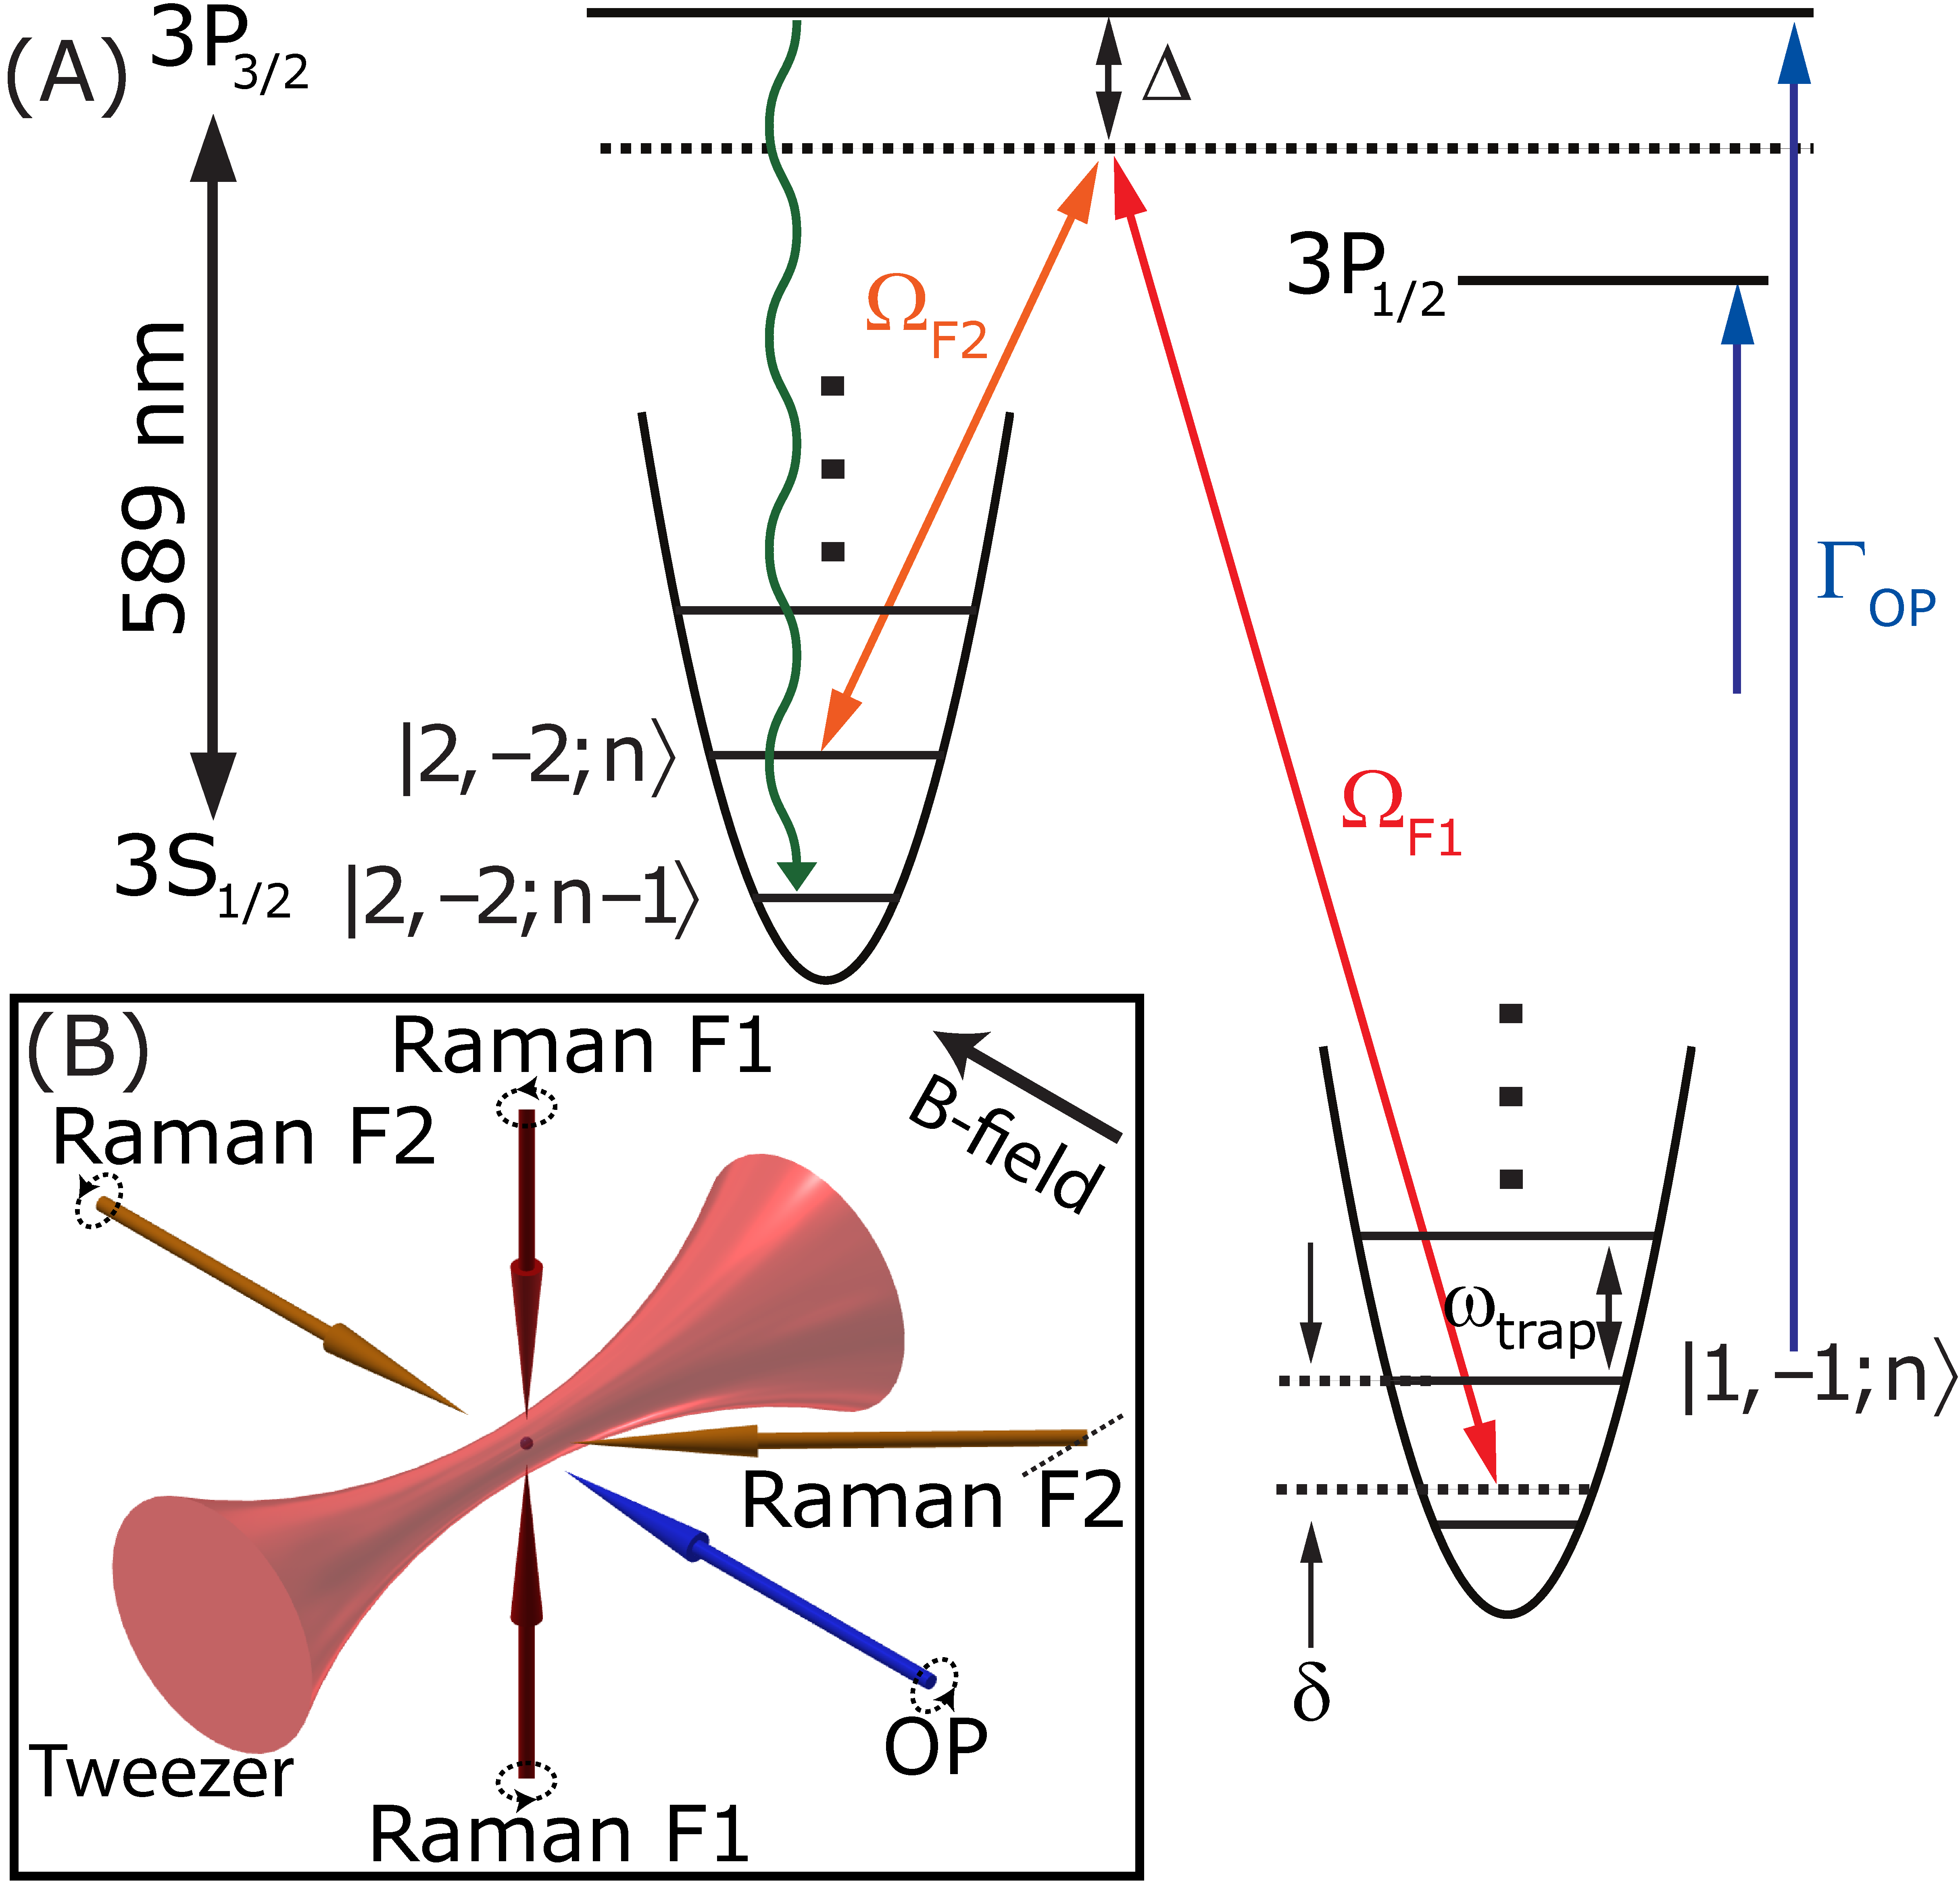
\includegraphics[height=5.2cm]{imgs/Na_RSC_schematic.pdf}
  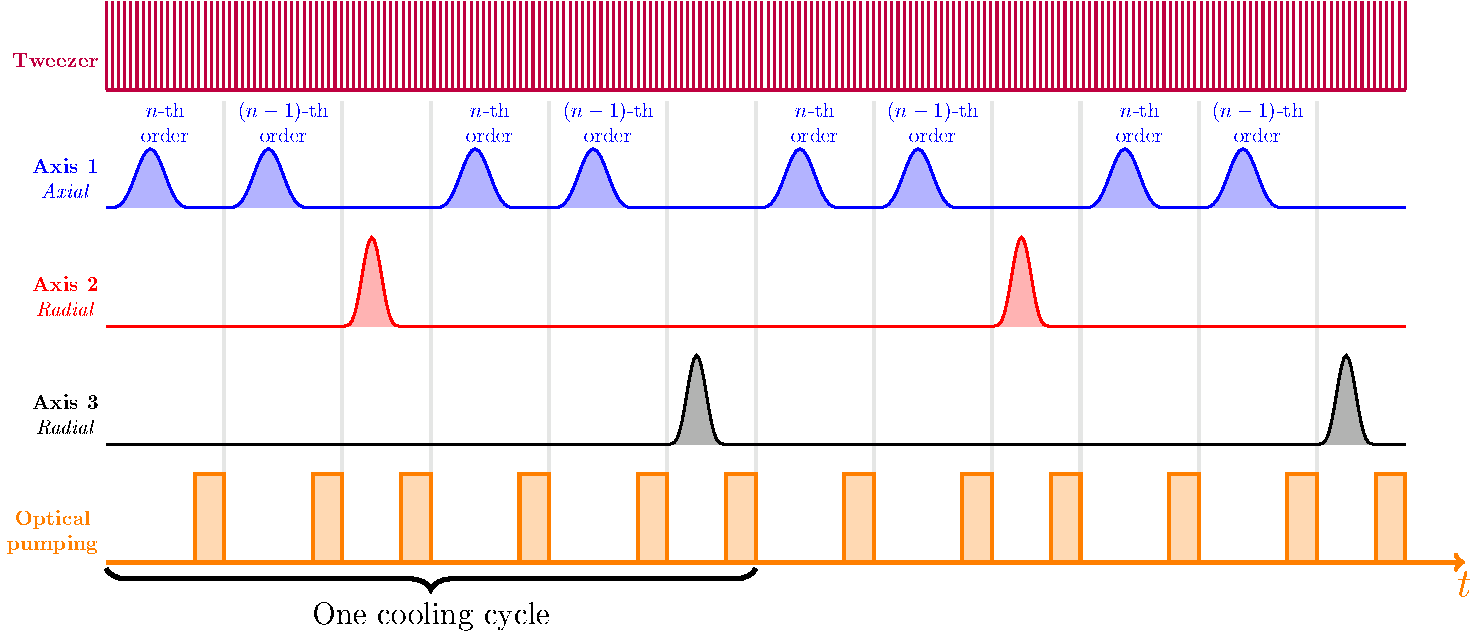
\includegraphics[height=4.5cm]{sequence.pdf}
  \caption{(A) Energy diagram. D1 OP
    (B) Beam directions and polarizations
    (C) Sequence description
    \label{f-setup}}
\end{figure*}
\begin{figure}[b]
  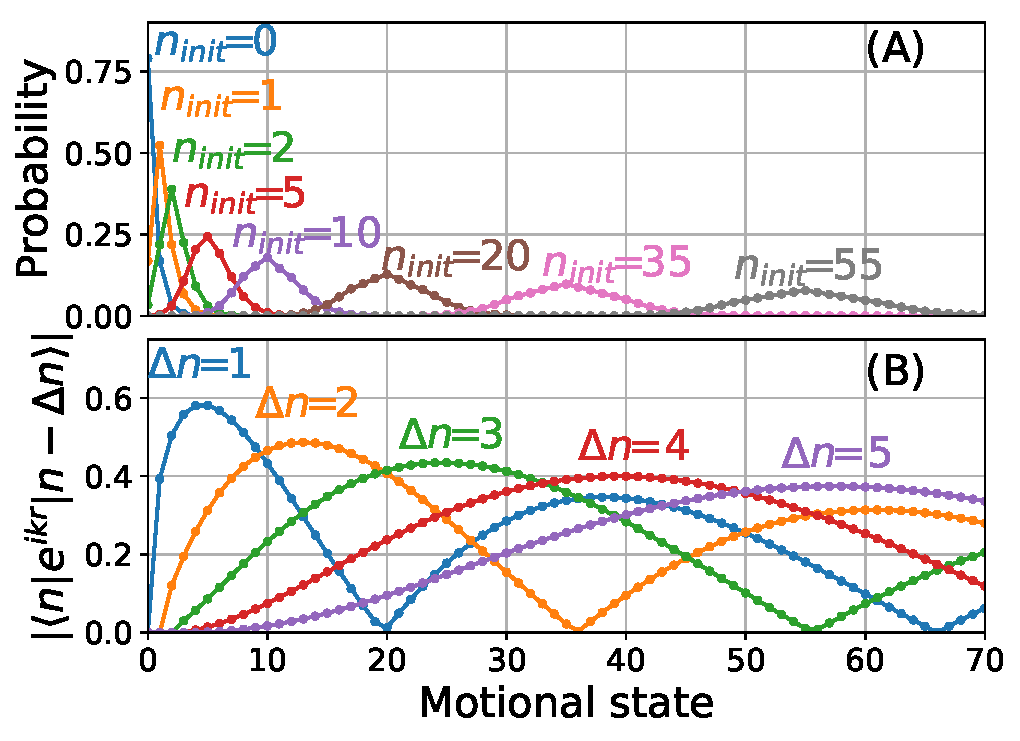
\includegraphics[width=8.5cm]{imgs/fig2_raman_op.pdf}
  \caption{Matrix elements and heating probabilities as a function of motional state.
    The range plotted covers $99\%$ of the initial thermal distribution.
    (A) Matrix elements for Raman transition in the axial direction showing diviation from
    $\sqrt{n}$ scaling and multiple minimums for different sideband orders.
    (B) Heating probability during the optical pumping step for all three axis.
    Due to the large Lamb-Dicke parameter,
    there is a high probability of heating especially in the axial direction.
    \label{f-ld}}
\end{figure}
\begin{figure*}
  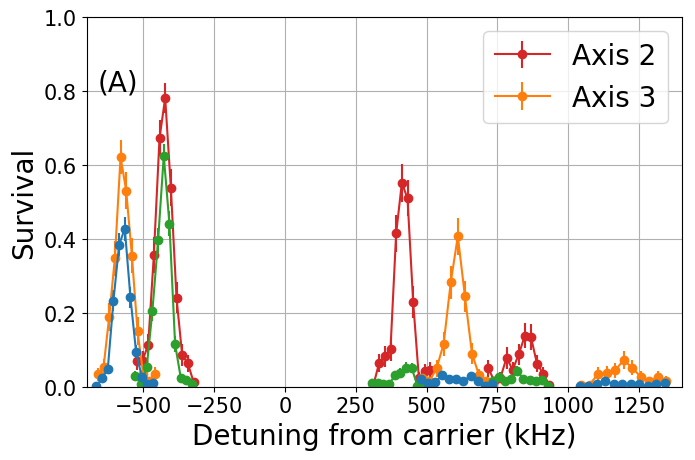
\includegraphics[width=8cm]{imgs/spectrum_r.png}
  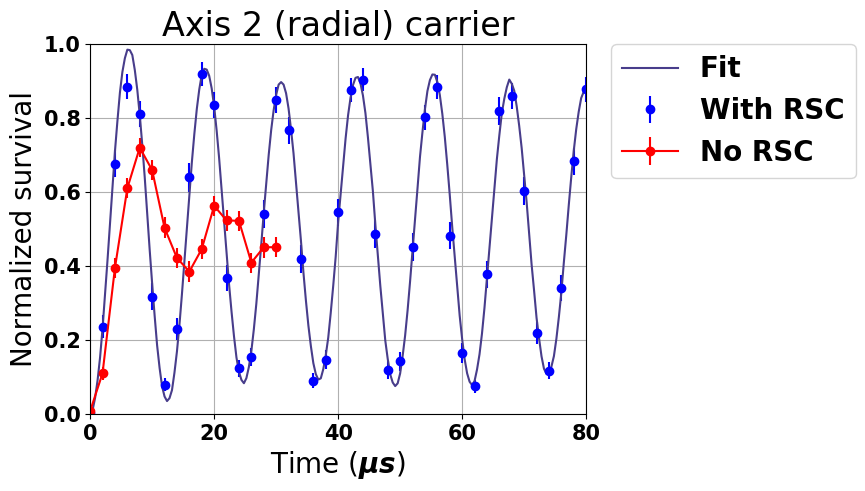
\includegraphics[width=8cm]{imgs/temp/fit_20170409_r2_0_ba.png}
  \caption{(A) (B) \label{f-radial}}
\end{figure*}
\begin{figure*}
  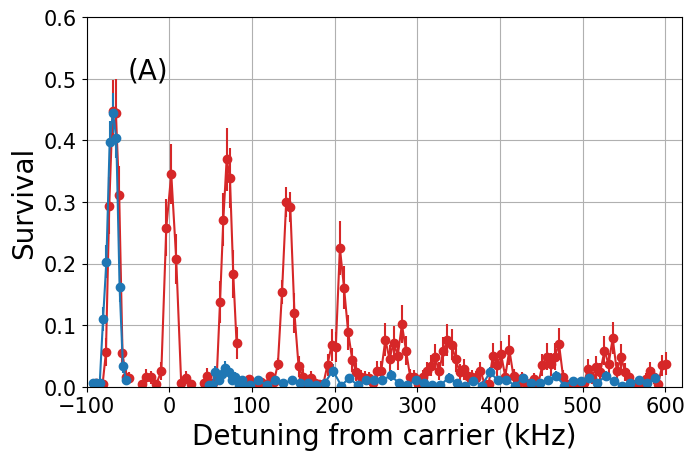
\includegraphics[width=8cm]{imgs/spectrum_a1.png}
  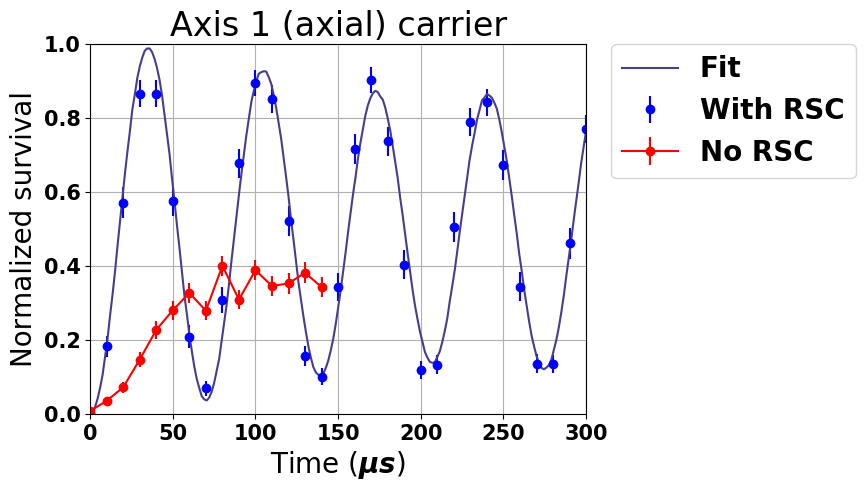
\includegraphics[width=8cm]{imgs/temp/fit_20170409_a1_0_ba.png}
  \caption{(A) (B) \label{f-axial}}
\end{figure*}

Single neutral atoms trapped in optical tweezers provide a promising system
for various applications including quantum information, quantum chemistry
and quantum simulation of many-body systems.
The interaction between different sites can be controlled by creating Rydberg excitation
or by creating dipolar molecules from two trapped atoms.
Combined with the ability to move, detect and manipulate individual sites,
arrays of optical tweezers can be used to prepare complex interacting system
with high fidelity.
In order to achieve long coherence time and full quantum control of the system needed for
these applications,
it is usually necessary to control the thermal motion of the atoms by cooling to the
three dimensional motional ground state in the optical tweezer,
which has already been demonstrated with heavy alkali atoms including rubidium and cesium.
However, some of the important properties of previous experiements,
for example low initial temperature and small Lamb-Dicke parameter,
may not be easily achievable for other systems and
the versatility of this approach requires being able to perform ground motional state cooling
in the more general case. In this letter, we present our work on cooling single sodium atoms
trapped in optical tweezers to the motional ground state with Raman sideband cooling.
Dispite having a large Lamb-Dicke parameter and high initial temperature,
by utilizing several new cooling techniques and a well optimized cooling sequence,
we are able to achieve a ground state probability of $80\%$.

The Raman sideband cooling we used to achieve the high ground state preparation fidelity
consists of multiple cycles of laser pulses to manipulate the internal and
motional states of the atoms.
Figure \ref{f-setup}A shows the schematic of the energy levels and the cooling sequence
in our setup.
Each cooling cycle starts with the Sodium atom in the $|F=2, m_F=-2\rangle$
ground electronic state and a certain vibration state $n$.
In the first step, a Raman pulse drives a transition to the motional state $n-\Delta n$
to reduce the motional energy while also changing the internal state to $|F=1, m_F=-1\rangle$.
In the second step, which finishes the cooling cycle,
an optical pumping pulse bring the atom back to the $|F=2, m_F=-2\rangle$ state to take away
the entropy. The second step could also change the motional state of the atoms which
could cause heating. The possibility for this to happen for an atom in the motional level $n$
is approximately proportional to the effective Lamb-Dicke parameter
$\eta^{OP}_{eff}=\sqrt{2n+1}\eta^{OP}$ where $\eta^{OP}=???$ is the Lamb-Dicke parameter for
optical pumping.
The geometry of the relevant beams (???and their polarizations) is showed in figure \ref{f-setup}B.
The optical tweezer has one weakly confined axial direction (axis $1$) and
two more strongly confined radial directions (axis $2$ and $3$).
Multiple pairs of beams are used to drive the Raman transition during cooling in order to
isolate and maximize the coupling to different trap axis.

Although Raman sideband cooling to motional ground state has already been successfully
implemented on neutral atoms in other experiments using heavier species like Rubidium [????]
and Cesium [????], such experiments generally use good polarization gradient cooling
and a tight confinement to achieve a small Lamb-Dicke parameter and effective Lamb-Dicke parameter.
However, this regime is harder to achieve with Sodium atoms, creating additional challenges for
us to realize ground state cooling. On the other hand, since these conditions can also be difficult
to meet for other interesting systems like directly laser cooled molecules, the techniques we
use to overcome these challenges could be useful for a wider variety of systems.

As mentioned previously, in order to perform Raman sideband cooling efficiently and
minimize the heating during the optical pumping, we need to have a low initial temperature and
a small Lamb-Dicke parameter. However, since the Lamb-Dicke parameter $\eta$ is inversely
proportional to $\sqrt{m}$ (???) where $m$ is the mass of the atom, it is larger for Sodium
given the same trap depth (???).
With $45mW$ of power at the focus of the trap, we measured a trapping frequency of
$\{\omega_1,\omega_2,\omega_3\}/2\pi = \{67, 420, 580\}\ \text{kHz}$
which corresponds to optical pumping Lamb-Dicke parameters of
$\{\eta^{OP}_1,\eta^{OP}_2,\eta^{OP}_3\} = \{???, ???, ???\}$.
Moreover, due to the unresolved(?) hyperfine structure in the $3^2P_{3/2}$ manifold,
the sub-Doppler cooling in Sodium is also less efficient and we start the
Raman sideband cooling with a initial temperature of $40\mu K$. Combined with the high Lamb-Dicke
parameters, this gives us a initial effective optical pumping Lamb-Dicke parameters of
$\{\eta^{OP}_{1eff},\eta^{OP}_{2eff},\eta^{OP}_{3eff}\} = \{???, ???, ???\}$
As a result, there is a very high probability of heating during the optical pumping step
(figure \ref{f-ld}B) causing a $30\%$ average heating probability during optical pumping
in the weakly confined axial direction. Fortunately, the high Lamb-Dicke parameters also
provide us tools to overcome this issue. From our geometry, the Lamb-Dicke parameters for
Raman transitions are $\{\eta^R_{1},\eta^R_{2},\eta^R_{3}\} = \{???, ???, ???\}$. As shown in
figure \ref{f-ld}A, the high Raman Lamb-Dicke parameters causes a strong coupling to higher orders
of cooling sidebands, especially for high motional states.
This enables us to cool atoms in high motional states by driving on high order Raman sidebands,
removing more motional energy in a single cooling pulse and offsetting the effect of
strong heating. Since the heating probability is higher for high motional states,
cooling on these high order sidebands can greatly suppress the high heating during
optical pumping during the initial cooling. Since the coupling strength of different orders
do not reach their minimums at the same time, using multiple orders of motional sidebands
for cooling also avoids accumulation of population near the coupling minimum of a particular
order, which improves the overall efficiency of the cooling process.

In additional to improving the cooling efficiency, the large Raman Lamb-Dicke parameters $\eta^R$
also creates difficulties for measuring the temperature. Traditional sideband thermometry uses
the ratio of the cooling and heating sidebands to measure $\bar n / (\bar n + 1)$, which relies
on the coupling strength to be proportional to $\sqrt{n}$. However, since we are not in the
Lamb-Dicke regime, the coupling strength deviates from this simple scaling rule quickly as already
shown in figure \ref{f-ld}A, causing the normal sideband thermometry to break down.
In order to solve this problem, when the atom temperature is still high,
we measure the heights of multiple sidebands to make sure no population is hidden at the
minimum of one sideband order. And when the atom is cooled down, we estimate the temperature
and ground state population under the assumption that only a few states are populated.
This result is then verified using independent measure of Rabi flopping on the carrier and heating
sidebands since they provide more information about the distribution of coupling strength.

Another issue caused by the high initial temperature is trap anharmonicity.
Although the potential near the center of a focused Gaussian beam can be approximated
by a harmonic trap, when a large number of levels are populated due to high initial temperature
the anharmonicity of the trap can lead to broadening of the sideband and decrease of
the sideband signal. In our setup, this effect limits the Rabi frequency of the Raman pulse
on the radial sidebands to be no lower than tens of kilo-Hertz in order to drive atoms in
different motional states equally.

Finally, the deep trap that is needed to trap and image single Sodium atom also creates
a very large AC Stark shift in the excited state. For the trap depth we are using, the
light shift in the center of the trap is as large as $300MHz$.
In additional to creating a large and position dependent detuning for the optical pumping light,
it also mixes the excited state state hyperfine levels,
affecting the branching ratio and increasing the number of photons needed during optical pumping.
Similar to our loading and imaging process [???], we solve this issue by switching the
trapping light at $3MHz$ during the whole cooling sequence.
Due to the large light shift, the optical pumping is effectively off when the trap light is on.
Since the atom can only be addressed by the optical pumping light when the trap light is off,
the effect of light shift on optical pumping fidelity is suppressed.

Taking all the features of our system into account, we use a Monte-Carlo simulation to verify
the validity of our method.
In the simulation, we can observe the high heating rate due to the high Lamb-Dicke parameters
and confirm that by using high order Raman sideband transition in the cooling sequence we can
suppress this effect and reduces the motional energy of the atom faster.
The simulation is also used to guide the optimization of the cooling sequence by exploring the
large parameter space and finding a robust cooling strategy. As shown in figure (?),
we found that instead of cooling on only one sideband order at a time, it is generally more
efficient to alternate the cooling pulse between two neighboring orders (axial) or pulse lengths.
A cooling sequence like this minimizes the accumulation of atom in a state not addressed by a
particular Raman pulse parameter.

For the more tightly confined radial directions,
we starts the cooling with $\{\bar n_2, \bar n_3\}=????, ????$.
The radial sideband spectra of the initial distribution is shown in figure \ref{f-radial}A
where we can clearly see the first order heating, first order cooling and
second order cooling sidebands.
After applying about 1000 cooling pulses cooling in all three dimensions
starting with cooling on the radial second order,
the Raman spectrum with the same parameter is shown in figure \ref{f-radial}B,
where the first and second order cooling sidebands on both axis are suppressed.
Given the absence of the second order cooling sideband,
we can estimate the ground state probability in each direction based on the height of
the first order cooling and heating sideband to be $????$ and $????$.
Due to the complexity of the sideband structure,
we measured the Rabi flopping on the carrier and heating sideband before and after cooling
(\ref{f-radial}C and \ref{f-radial}D)
as a independent way to obtain the population in different motional states.
Fitting the Rabi flopping data give a ground state probability of $????$ and $????$,
showing good agreement between the two methods.

The axial direction is much less confined and therefore has a much higher initial effective
Lamb-Dicke parameter of $\eta^{OP}_{eff1}\approx3.3$.
The line in figure \ref{f-axial}A shows the Raman spectrum in the axial direction
before applying Raman sideband cooling where we can see clearly resolved Raman cooling sidebands
up to the eighth order suggesting that we have many motional states populated in this direction.
Therefore, we starts our cooling sequence by driving Raman transitions on the eighth order axial
cooling sideband. After applying the cooling sequence identical to the one we use to cool
the radial directions, the spectrum is shown as the blue line in figure \ref{f-axial}A.
All of the high order ($\geqslant2$) axial cooling sidebands disappeared and the first order
cooling sideband is also strongly suppressed.
The ground state probability calculated from this spectrum is $????$.
We can also use Rabi flopping on the carrier and heating sideband to varify this result
similar to the radial direction. In this case, we see very good agreement on the carrier
(figure \ref{f-axial}B) but there is additional decoherence on the axial first order
heating sideband (figure \ref{f-axial}C).
We believe this decoherence is caused by technical noise in our setup which
produces the strongest effect on this transition due to its slow Rabi frequency.
The decoherence time scale agree with the magnetic field fluctuation we measured which produces
a Zeeman shift of around $5kHz$.

% Missing:
% ?? D1 OP
% ?? Blackman pulse

\bibliography{paper}
\end{document}
